% This is LLNCS.DEM the demonstration file of
% the LaTeX macro package from Springer-Verlag
% for Lecture Notes in Computer Science,
% version 2.4 for LaTeX2e as of 16. April 2010
%
\documentclass{llncs}
%
\usepackage{makeidx}  % allows for indexgeneration
\usepackage[hidelinks]{hyperref}
\usepackage{graphicx}
%
\begin{document}
%
\frontmatter          % for the preliminaries
%
\pagestyle{headings}  % switches on printing of running heads
%
\mainmatter              % start of the contributions
%
\title{Solving the Expression Problem for LTL using Object Algebra}
%
\titlerunning{Solving the Expression Problem for LTL using Object Algebra}  % abbreviated title (for running head)
%                                     also used for the TOC unless
%                                     \toctitle is used
%
\author{Ren\'e Kremer%\inst{1}%\orcidID{0000-1111-2222-3333}
\and
Hannes Kallwies%\inst{2}%\orcidID{1111-2222-3333-4444} 
\and
Simon Thiessen%\orcidID{2222-3333-4444-5555}
}
%
\authorrunning{Ren\'e Kremer et al.} % abbreviated author list (for running head)
%
%%%% list of authors for the TOC (use if author list has to be modified)
\tocauthor{Ren\'e Kremer, Hannes Kallwies, Simon Thiessen}
%
\institute{Institute for Software Engineering and Programming Languages, Universit\"at zu L\"ubeck, L\"ubeck, Germany\\
\email{rene.kremer@student.uni-luebeck.de} \\
\email{hannes.kallwies@student.uni-luebeck.de} \\
\email{simon.thiessen@student.uni-luebeck.de}}

\maketitle              % typeset the title of the contribution

\begin{abstract}
The expression problem, as described in \cite{wadler}, describes the problem of defining data types, which can be extended with new data types and new functions without recompiling existing code and retaining static type safety. This lead to some pattern, which handle the problem more or less well. In this paper we will discuss the use of object algebra instead of patterns like the interpreter or visitor pattern. We will use Linear Temporal Logic (LTL) \cite{pnueli} as an example to show how one can use object algebra to solve the expression problem. For this case we start with a given set of LTL expressions and an evaluation function. In the process we extend our LTL object algebra by a new data type and new function.
\keywords{expression problem, visitor pattern, interpreter pattern, object algebra}
\end{abstract}
%
\section{Introduction} \label{sec:introduction}
The expression problem was coined by Philip Wadler in \cite{wadler} and describes a problem, which can be used to benchmark the expressiveness of programming language by a question like "how much can your language express?". The expression problem therefore discusses strengths and weaknesses of programming languages and paradigms.

Philip Wadler presented in \cite{wadler} the goal to define data types that could be extended by new cases of data types and new functions, while retaining static type safety and without recompiling existing code.

There are different approaches to solve the expression problem, e.g. the visitor pattern and interpreter pattern, which will be introduced in \autoref{sec:approaches}. As with nearly everything each approach has it's two sides of a coin. 

The expression problem itself can be part of different kind of practical problems one needs to solve. One can reduce string matching to regular expressions, which can be reduced to the expression problem. Therefore the interpreter pattern would suggest different classes for expression likes \emph{literal}, \emph{alternation} and \emph{repetition} as shown in \cite{GHJV}.

In practical terms regular expression will mostly be modeled via a state machine and not with more or less complex expression classes. But one could easy come up with his or hers own grammar which needs to be interpreted to get the information it expresses, e.g. the commandos of RoboCups Soccer server\footnote{http://www.robocup.org/}.

In \autoref{sec:approaches} we will give more insight about the visitor and interpreter patterns but also about object algebra. \autoref{sec:oa-ltl} will describe our approach using object algebra with the given set of LTL expressions and their extended types and functions. The paper ends in \autoref{sec:conclusion} with a conclusion about the strengths and weaknesses of object algebra in comparison to the visitor and interpreter pattern.

\section{Approaches to the expression problem} \label{sec:approaches}
In this section we will give a short overview how the patterns work for a comparison later on. We will start with the interpreter pattern in \autoref{ssec:interpreter}, move to the visitor pattern in \autoref{ssec:visitor} and finish this section with object algebra in \autoref{ssec:oa}.

\subsection{Interpreter Pattern} \label{ssec:interpreter}
The interpreter pattern is used if a kind of problem occurs often enough. Instances of the problem will then be expressed in a simple language. The interpreter can then solve the problem by interpreting the sentences of the language.

In object-oriented languages this can be done by writing classes which represent expressions of the language. \cite{GHJV} uses the language for regular expressions as an example.

Therefore every regular expression can be represented by its grammar in an abstract syntax tree (AST), which is made up of the instances of the expression classes. An example AST is shown in \autoref{fig:interpreter-pattern-ast}.

\begin{figure}[h]
	\centering
	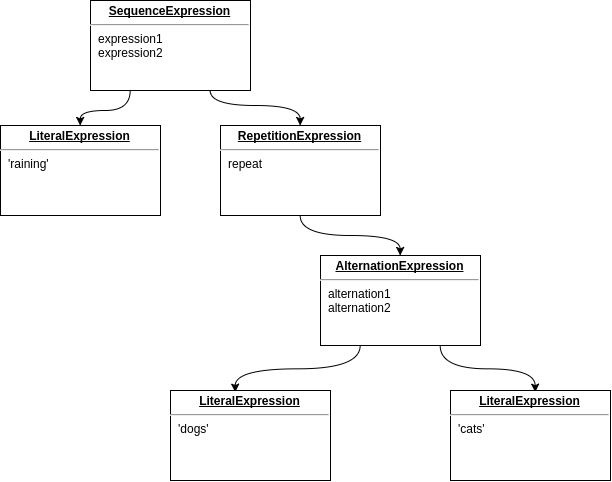
\includegraphics[width=\textwidth]{img/Interpreter-Pattern-AST-Example}
	\caption{Example in \cite{GHJV} for the AST of regular expressions using the interpreter pattern }
	\label{fig:interpreter-pattern-ast}
\end{figure} 

Operations on these expression classes will be implemented in the class. So if we want to evaluate an expression each node evaluates itself with the defined operation.

The following benefits and liabilities are described in \cite{GHJV}:

\begin{description}
	\item[It's easy to change and extend the grammer:] Using classes to represent grammar rules allows to use inheritance to extend the grammer. New data types will be derived from existing ones.
	\item[Implementing the grammer is easy, too:] The nodes of the AST have similar implementation, which makes the implementation easy and repetitive This process can be automated with compiler or parser generators.
	\item[Complex grammars are hard to maintain:] At least one class is defined for every expression. This means that complex grammars have many different classes, which needs to be maintained. Adding a new operation on these classes means you need to change every class accordingly.
\end{description}

So as one can see the interpreter is great for grammars that are rather simple and don't change that much. Extending the grammer is easy, but adding new operations is not. Object algebra uses the terms \emph{data variation} and \emph{operations}. Using these terms one can briefly summarize the interpreter as a good way to handle data variations to a certain extend (not too complex grammars), but adding new operations to expressions can easily lead to many changes as every class of each expression needs an implementation of the new operation. This means that every expression class will be edited.



\subsection{Visitor Pattern} \label{ssec:visitor}
\subsection{Object Algebra} \label{ssec:oa}
\section{Object Algebra to the LTL Expression Problem} \label{sec:oa-ltl}
\section{Conclusion} \label{sec:conclusion}

%
% ---- Bibliography ----
%
\begin{thebibliography}{5}
%

\bibitem{wadler}
Wadler, P.:
The Expression Problem.
E-Mail Discussion (1998),
\url{http://homepages.inf.ed.ac.uk/wadler/papers/expression/expression.txt}

\bibitem{pnueli}
Pnueli, A.:
The temporal logic of programs.
In 18th Annual Symposium on Foundations of Computer Science, Providence, Rhode Island, USA, 31 October - 1 November 1977, pages 46-57, IEEE Computer Society, 1977

\bibitem{GHJV}
Gamma, E., Helm R., Johnson R. and Vlissides J.:
Design Patterns: Elements of Reusable Object-Oriented Software.
Addison-Wesley Professional Computing Series, Pearson Education, 1994
%\bibitem {clar:eke}
%Clarke, F., Ekeland, I.:
%Nonlinear oscillations and
%boundary-value problems for Hamiltonian systems.
%Arch. Rat. Mech. Anal. 78, 315--333 (1982)

%\bibitem {clar:eke:2}
%Clarke, F., Ekeland, I.:
%Solutions p\'{e}riodiques, du
%p\'{e}riode donn\'{e}e, des \'{e}quations hamiltoniennes.
%Note CRAS Paris 287, 1013--1015 (1978)
%
%\bibitem {mich:tar}
%Michalek, R., Tarantello, G.:
%Subharmonic solutions with prescribed minimal
%period for nonautonomous Hamiltonian systems.
%J. Diff. Eq. 72, 28--55 (1988)
%
%\bibitem {tar}
%Tarantello, G.:
%Subharmonic solutions for Hamiltonian
%systems via a $\bbbz_{p}$ pseudoindex theory.
%Annali di Matematica Pura (to appear)
%
%\bibitem {rab}
%Rabinowitz, P.:
%On subharmonic solutions of a Hamiltonian system.
%Comm. Pure Appl. Math. 33, 609--633 (1980)

\end{thebibliography}
\end{document}
